\section{Axiomatisation of Interval Algebras}
\label{sec:axiomatisation}

\begin{defn}
  We define the language of strict linear orders $\lslo$ as the single binary relation $\{ < \}$.

  We define the theory of strict linear orders as
  \begin{align*}
    \tslo = \{ & \forall a, \lnot\ (a < a), \\
              & \forall a, \forall b, \forall c, (a < b) \land (b < c) \rightarrow (a < c) \\
              & \forall a, \forall b, (a < b) \lor (a = b) \lor (b < a) \}
  \end{align*}
\end{defn}

\begin{defn}
  We define the language of Allen interval algebras $\laia$ as
  \begin{equation*}
    \laia = \{ \before, \meets, \overlaps, \starts, \finishes, \contained,
               \after, \metby, \overlappedby, \startedby, \finishedby, \contains \}
  \end{equation*}

  {\color{orange} TODO write out the axioms of interval algebras}
\end{defn}

{\color{orange} TODO show it suffices to consider relations of the form -> when showing a function
is an embedding}
% mention how we only need to prove the forward implication to show something is a
% $\laia$-embedding. This is enough since the relations are mutually-exclusive and exhaustive.
% Also it is enough to check that the relations of the form -> are preserved -- if that is the case
% then the relations of the form <- are automatically also preserved by "duality"?/"symmetry"?

% ------ Justifying this axiomatisation of interval algebras

\begin{defn}
  Given a linear order $L$ we define its set of non-zero intervals $\inter[P]$ as the set
  \begin{equation*}
    \inter[L] = \left\{(x_1,x_2)\ |\ x_1 < x_2 \right\} \subseteq L^2
  \end{equation*}
  We can turn this into a $\laia$-structure under the interpretations:
  \begin{itemize}
    \item $(x_1,x_2) \aiaarrow{i} (y_1,y_2)$ if and only if
      $L \models \defformula{\aiaarrow{i}}(x_1,x_2,y_1,y_2)$.
    \item $(x_1,x_2) \raiaarrow{i} (y_1,y_2)$ if and only if
      $L \models \defformula{\aiaarrow{i}}(y_1,y_2,x_1,x_2)$.
  \end{itemize}
  where we range $i$ over the indexing set $\aiaindex$ and define the first order
  $\lslo$-formulas by
  \begin{align*}
    \beforef(x_1,x_2,y_1,y_2)    & = \left(x_1 < x_2\right) \land \left(x_2 < y_1\right) \land
      \left(y_1 < y_2\right) \\
    \meetsf(x_1,x_2,y_1,y_2)     & = \left(x_1 < x_2\right) \land \left(x_2 = y_1\right) \land
      \left(y_1 < y_2\right) \\
    \overlapsf(x_1,x_2,y_1,y_2)  & = \left(x_1 < y_1\right) \land \left(y_1 < x_2\right) \land
      \left(x_2 < y_2\right) \\
    \startsf(x_1,x_2,y_1,y_2)    & = \left(x_1 = y_1\right) \land \left(y_1 < x_2\right) \land
      \left(x_2 < y_2\right) \\
    \finishesf(x_1,x_2,y_1,y_2)  & = \left(y_1 < x_1\right) \land \left(x_1 < x_2\right) \land
      \left(x_2 = y_2\right) \\
    \containedf(x_1,x_2,y_1,y_2) & = \left(y_1 < x_1\right) \land \left(x_1 < x_2\right) \land
      \left(x_2 < y_2\right) \\
  \end{align*}
\end{defn}

\begin{thm}
  Given a strict linear order $L$, $\inter[L]$ is a model of $\taia$ under the above
  interpretations.
\end{thm}
\begin{proof}
  {\color{orange} TODO Tedious proof by cases goes here}
\end{proof}

\begin{cor}
  Allen's interval algebras are satisfiable
\end{cor}

The theory is satisfiable in a reasonable way, including the expected models induced from linear
orders. To further support this tight connection, we see interval algebras also induce a quite
reasonable linear order

\begin{defn}
  Given an Allen interval algebra $A$, we define $\points[A] = \frac{A + A}{\psim}$ where
  $\psim$ is an equivalence relation on the set $A + A$ defined by
  \begin{equation*}
    (n,I) \psim (m,J) \iff A \models \peq(n,m)(I,J)
  \end{equation*}
  Where $\peq$ assigns $\laia$-formulas with open variables $I,J$ to pairs $(n,m) \in \{0,1\}^2$
  \begin{equation*}
    \peq(n,m)(I,J) = \begin{cases}
      I \starts J \lor I \startedby J \lor I = J \quad & \text{if } n = m = 0 \\
      I \finishes J \lor I \finishedby J \lor I = J    & \text{if } n = m = 1 \\
      I \metby J                                       & \text{if } n = 0,\ m = 1 \\
      I \meets J                                       & \text{if } n = 1,\ m = 0
    \end{cases}
  \end{equation*}
\end{defn}

{\color{orange} TODO at least add a remark why this is an equivalence relation}

\begin{thm}
  Given an Allen interval algebra $A$, the interpretation of the symbol $<$ in $\points[A]$ given by
  $[(n,I)] < [(m,J)] \iff A \models \plt(n,m)(I,J)$ is well-defined and turns $A$ into a model of
  $\tslo$.

  Here, $\plt$ is a function assigning $\laia$-formulas with open variables $I,J$ to pairs
  $(n,m) \in \{0,1\}^2$ defined as:
  \begin{equation*}
    \plt(n,m)(I,J) = \begin{cases}
      (I \before J) \lor (I \meets J) \lor (I \overlaps J)  \lor (I \finishedby J)
                    \lor (I \contains J)        & \text{if } n = m = 0\\
      (I \before J) \lor (I \meets J) \lor (I \overlaps J) \lor (I \starts J)
                  \lor (I \contained J)         & \text{if } n = m = 1 \\
      \lnot\,(I \after J) \land \lnot\,(I \metby J)
                                                & \text{if } n = 0,\ m = 1 \\
      I \before J                               & \text{if } n = 1,\ m = 0
    \end{cases}
  \end{equation*}
\end{thm}
\begin{proof}
  First we must check that this ordering relation on $\points[A]$ is well-defined. For this fix
  intervals $I_1,I_2,J_1,J_2 \in A$ and $n_1,n_2,m_1,m_2 \in \{0,1\}$ and assume that
  \begin{equation*}
    [(n_1,I_1)] = [(n_2,I_2)] < [(m_2,J_2)] = [(m_1,J_1)]
  \end{equation*}
  Then we must show that indeed, $[(n_1,I_1)] < [(m_1,J_1)]$. There are 16 distinct cases which
  we cover in \cref{tab:plt_well_defined}. Since, in each of the cases, with the possible relations
  $I_1 \longrightarrow J_1$ found in the last column, it is definitely the case that
  $A \models \plt(n_1,m_1)(I_1,J_1)$.

  \begin{table}[ht]
    \centering
    \setlength\extrarowheight{5pt}
    \begin{tabular}{|c|c|c|}
      \hline
      $(n_1,n_2,m_1,m_2)$ & Relation between $I_1,I_2,J_1,J_2$ & Relation between $I_1,J_1$ \\
      \hline\hline
      $(0,0,0,0)$ & $I_1 \aiaarrow{s=S} I_2 \aiaarrow{<moFD} J_2 \aiaarrow{s=S} I_1$ &
        $I_1 \aiaarrow{<moFD} J_1$ \\\hline
      $(0,0,0,1)$ & $I_1 \aiaarrow{s=S} I_2 \aiaarrow{<mosfd=OSFD} J_2 \aiaarrow{m} I_1$ &
        $I_1 \aiaarrow{<moFD} J_1$ \\\hline
      $(0,0,1,0)$ & $I_1 \aiaarrow{s=S} I_2 \aiaarrow{<moFD} J_2 \aiaarrow{M} I_1$ &
        $I_1 \aiaarrow{<mosfd=OSFD} J_1$ \\\hline
      $(0,0,1,1)$ & $I_1 \aiaarrow{s=S} I_2 \aiaarrow{<mosfd=OSFD} J_2 \aiaarrow{f=F} I_1$ &
        $I_1 \aiaarrow{<mosfd=OSFD} J_1$ \\\hline
      $(0,1,0,0)$ & $I_1 \aiaarrow{M} I_2 \aiaarrow{<} J_2 \aiaarrow{s=S} I_1$ &
        $I_1 \aiaarrow{<moFD} J_1 $ \\\hline
      $(0,1,0,1)$ & $I_1 \aiaarrow{M} I_2 \aiaarrow{<mosd} J_2 \aiaarrow{m} I_1$ &
        $I_1 \aiaarrow{<moFD} J_1 $ \\\hline
      $(0,1,1,0)$ & $I_1 \aiaarrow{M} I_2 \aiaarrow{<} J_2 \aiaarrow{M} I_1$ &
        $I_1 \aiaarrow{<mosfd=OSFD} J_1$ \\\hline
      $(0,1,1,1)$ & $I_1 \aiaarrow{M} I_2 \aiaarrow{<mosd} J_2 \aiaarrow{f=F} I_1$ &
        $I_1 \aiaarrow{<mosfd=OSFD} J_1$ \\\hline
      $(1,0,0,0)$ & $I_1 \aiaarrow{m} I_2 \aiaarrow{<moFD} J_2 \aiaarrow{s=S} I_1$ &
        $I_1 \aiaarrow{<} J_1$ \\\hline
      $(1,0,0,1)$ & $I_1 \aiaarrow{m} I_2 \aiaarrow{<mosfd=OSFD} J_2 \aiaarrow{m} I_1$ &
        $I_1 \aiaarrow{<} J_1$ \\\hline
      $(1,0,1,0)$ & $I_1 \aiaarrow{m} I_2 \aiaarrow{<moFD} J_2 \aiaarrow{M} I_1$ &
        $I_1 \aiaarrow{<mosd} J_1$ \\\hline
      $(1,0,1,1)$ & $I_1 \aiaarrow{m} I_2 \aiaarrow{<mosfd=OSFD} J_2 \aiaarrow{f=F} I_1$ &
        $I_1 \aiaarrow{<mosd} J_1$ \\\hline
      $(1,1,0,0)$ & $I_1 \aiaarrow{f=F} I_2 \aiaarrow{<} J_2 \aiaarrow{s=S} I_1$ &
        $I_1 \aiaarrow{<} J_1$ \\\hline
      $(1,1,0,1)$ & $I_1 \aiaarrow{f=F} I_2 \aiaarrow{<mosd} J_2 \aiaarrow{m} I_1$ &
        $I_1 \aiaarrow{<} J_1$ \\\hline
      $(1,1,1,0)$ & $I_1 \aiaarrow{f=F} I_2 \aiaarrow{<} J_2 \aiaarrow{M} I_1$ &
        $I_1 \aiaarrow{<mosd} J_1$ \\\hline
      $(1,1,1,1)$ & $I_1 \aiaarrow{f=F} I_2 \aiaarrow{<mosd} J_2 \aiaarrow{f=F} I_1$ &
        $I_1 \aiaarrow{<mosd} J_1$ \\\hline
    \end{tabular}
    \caption{
      All cases to check if the ordering on $\points[A]$ is well defined.
    }
    \label{tab:plt_well_defined}
  \end{table}

  Now we know that our definition of $<$ does not depend on a choice of representative, we need
  to check whether it satisfies $\tslo$:
  \begin{itemize}
    \item \textbf{irreflexivity}: Fix some element $[(n,I)] \in \points[A]$. Since the interval
      algebra relations (along with equality) are mutually exclusive and $I = I$, no other relation
      can hold for the pair $(I,I)$. Regardless of the value of $n$, $\plt(n,n)(I,I)$ does not
      include $I = I$ as a disjunct, so $A \not\models \plt(n,n)(I,I)$ and $<$ is irreflexive.
    \item \textbf{transitivity}: To show transitivity we start by fixing intervals $I,J,K \in A$ and
      assuming that $[(n,I)] < [(m,J)]$ and $[(m,J)] < [(l,K)]$. Then there are 8 cases
      based on the values of $n,m,k \in \{0,1\}$, all of which are considered in
      \cref{tab:plt_trans_000} up to \cref{tab:plt_trans_111}.
    \item \textbf{trichotomy}: Fix two $I,J \in A$. To check the trichotomy condition holds, we need
      to show that for all $n,m \in \{0,1\}$ we have
      \begin{equation*}
        A \models \plt(n,m)(I,J) \lor \peq(n,m)(I,J) \lor \plt(m,n)(J,I)
      \end{equation*}
      There are 3 cases that we must deal with separately to show this:
      \begin{itemize}
        \item First we consider $[(0,I)]$ and $[(0,J)]$. The formula $\plt(0,0)(I,J)$ is a
          disjunction 5 of our basic relations and $\plt(0,0)(J,I)$ the disjunction of its duals.
          Then $\peq(0,0)(I,J)$ is a disjunction of the 2 missing relations and equality. Hence by
          exhaustiveness of the interval algebra relations and equality, it must be the case that
          $A \models \plt(0,0)(I,J) \lor \peq(0,0)(I,J) \lor \plt(0,0)(J,I)$
        \item Next, we consider $[(0,I)]$ and $[(1,J)]$. The formula $\plt(0,1)(I,J)$ is a
          conjunction of 2 negated relational symbols, which is equivalent to the disjunction of
          equality and the 10 absent relations. Then $\peq(0,1)(I,J) \lor \plt(1,0)(J,I)$ is the
          disjunction of the two missing relations.
        \item Finally we consider $[(1,I)]$ and $[(1,J)]$. The situation here is similar to the
          $n = m = 0$ case, since $\plt(1,1)(I,J)$ is a disjunction of 5 basic relations, then
          $\plt(1,1)(J,I)$ is the disjunction of its duals and $peq(1,1)(I,J)$ is the disjunction
          of the 2 missing relations and equality.
      \end{itemize}
      When $(n,m)=(1,0)$, since $\psim$ is symmetric, we know that
      \begin{equation*}
        A \models \peq(1,0)(I,J) \iff A \models \peq(0,1)(J,I)
      \end{equation*}
      which allows us to reduce to the second case above.
  \end{itemize}
\end{proof}

{\color{orange} TODO acknowledge that this is not an interpretation generally.}

{\color{blue} TODO Consider adding table justifying these definitions? Something like:

| I relation J | drawing of I and J | is I- less than J- | is I+ lt J+ | is I- lt J + | is I+ lt J - |}



{\color{orange} TODO figure out whether or not to keep this.

Now that this axiomatisation is justified, show that we can't remove any axioms without making
it into something we do not want.}

% 0 0 0 case
\begin{table}[ht]
  \centering
  \begin{tabular}{| c | c | c || c | c | c || c | c | c |}
    \hline
    $I \to J$ & $J \to K$ & $I \to K$ &
      $I \to J$ & $J \to K$ & $I \to K$ &
      $I \to J$ & $J \to K$ & $I \to K$ \\
    \hline\hline
    \llrow & \olrow & \Dlrow \\
    \lmrow & \omrow & \Dmrow \\
    \lorow & \oorow & \Dorow \\
    \lFrow & \oFrow & \DFrow \\
    \lDrow & \oDrow & \DDrow \\
    \hline
    \mlrow & \Flrow &&&\\
    \mmrow & \Fmrow &&&\\
    \morow & \Forow &&&\\
    \mFrow & \FFrow &&&\\
    \mDrow & \FDrow &&&\\
    \hline
  \end{tabular}
  \caption{
    The transitivity table for the $\istart{I} < \istart{J}$ and $\istart{J} < \istart{K}$ case.
    For this to imply $\istart{I} < \istart{K}$ we need the $I \to K$ columns to all contain a
    subset of the string $<moFD$.
  }
  \label{tab:plt_trans_000}
\end{table}

% 0 0 1 case
\begin{table}[ht]
  \centering
  \begin{tabular}{| c | c | c || c | c | c || c | c | c |}
    \hline
    $I \to J$ & $J \to K$ & $I \to K$ &
      $I \to J$ & $J \to K$ & $I \to K$ &
      $I \to J$ & $J \to K$ & $I \to K$ \\
    \hline\hline
    \llrow & \olrow & \Dlrow \\
    \lmrow & \omrow & \Dmrow \\
    \lorow & \oorow & \Dorow \\
    \lsrow & \osrow & \Dsrow \\
    \lfrow & \ofrow & \Dfrow \\
    \ldrow & \odrow & \Ddrow \\
    \lerow & \oerow & \Derow \\
    \lOrow & \oOrow & \DOrow \\
    \lSrow & \oSrow & \DSrow \\
    \lFrow & \oFrow & \DFrow \\
    \lDrow & \oDrow & \DDrow \\
    \hline
    \mlrow & \Flrow &&&\\
    \mmrow & \Fmrow &&&\\
    \morow & \Forow &&&\\
    \msrow & \Fsrow &&&\\
    \mfrow & \Ffrow &&&\\
    \mdrow & \Fdrow &&&\\
    \merow & \Ferow &&&\\
    \mOrow & \FOrow &&&\\
    \mSrow & \FSrow &&&\\
    \mFrow & \FFrow &&&\\
    \mDrow & \FDrow &&&\\
    \hline
  \end{tabular}
  \caption{
    The transitivity table for the $\istart{I} < \istart{J}$ and $\istart{J} < \iend{K}$ case.
    For this to imply $\istart{I} < \iend{K}$ we need the $I \to K$ columns to all contain a
    subset of the string $<mosfd=OSFD$. Recall that concur is shorthand for $osfd=OSFD$
  }
  \label{tab:plt_trans_001}
\end{table}


% 0 1 0 case
\begin{table}[ht]
  \centering
  \begin{tabular}{| c | c | c |}
    \hline
    $I \to J$ & $J \to K$ & $I \to K$ \\
    \hline\hline
    \llrow \\
    \mlrow \\
    \olrow \\
    \slrow \\
    \flrow \\
    \dlrow \\
    \elrow \\
    \Olrow \\
    \Slrow \\
    \Flrow \\
    \Dlrow \\
    \hline
  \end{tabular}
  \caption{
    The transitivity table for the $\istart{I} < \iend{J}$ and $\iend{J} < \istart{K}$ case.
    For this to imply $\istart{I} < \istart{K}$ we need the $I \to K$ columns to all contain a
    subset of the string $<mofD$.
  }
  \label{tab:plt_trans_010}
\end{table}

% 0 1 1 case
\begin{table}[ht]
  \centering
  \begin{tabular}{| c | c | c || c | c | c || c | c | c |}
    \hline
    $I \to J$ & $J \to K$ & $I \to K$ &
      $I \to J$ & $J \to K$ & $I \to K$ &
      $I \to J$ & $J \to K$ & $I \to K$ \\
    \hline\hline
    \llrow & \flrow & \Slrow \\
    \lmrow & \fmrow & \Smrow \\
    \lorow & \forow & \Sorow \\
    \lsrow & \fsrow & \Ssrow \\
    \ldrow & \fdrow & \Sdrow \\
    \hline
    \mlrow & \dlrow & \Flrow \\
    \mmrow & \dmrow & \Fmrow \\
    \morow & \dorow & \Forow \\
    \msrow & \dsrow & \Fsrow \\
    \mdrow & \ddrow & \Fdrow \\
    \hline
    \olrow & \elrow & \Dlrow \\
    \omrow & \emrow & \Dmrow \\
    \oorow & \eorow & \Dorow \\
    \osrow & \esrow & \Dsrow \\
    \odrow & \edrow & \Ddrow \\
    \hline
    \slrow & \Olrow &&&\\
    \smrow & \Omrow &&&\\
    \sorow & \Oorow &&&\\
    \ssrow & \Osrow &&&\\
    \sdrow & \Odrow &&&\\
    \hline
  \end{tabular}
  \caption{
    The transitivity table for the $\istart{I} < \iend{J}$ and $\iend{J} < \iend{K}$ case.
    For this to imply $\istart{I} < \iend{K}$ we need the $I \to K$ columns to all contain a
    subset of the string $<mosfd=OSFD$. Recall that concur is shorthand for $osfd=OSFD$.
  }
  \label{tab:plt_trans_011}
\end{table}

% 1 0 0 case
\begin{table}[ht]
  \centering
  \begin{tabular}{| c | c | c |}
    \hline
    $I \to J$ & $J \to K$ & $I \to K$ \\
    \hline\hline
    \llrow \\
    \lmrow \\
    \lorow \\
    \lFrow \\
    \lDrow \\
    \hline
  \end{tabular}
  \caption{
    The transitivity table for the $\iend{I} < \istart{J}$ and $\istart{J} < \istart{K}$ case.
    For this to imply $\iend{I} < \istart{K}$ we need the $I \to K$ columns to all contain $<$.
  }
  \label{tab:plt_trans_100}
\end{table}

% 1 0 1 case
\begin{table}[ht]
  \centering
  \begin{tabular}{| c | c | c |}
    \hline
    $I \to J$ & $J \to K$ & $I \to K$ \\
    \hline\hline
    \llrow \\
    \lmrow \\
    \lorow \\
    \lsrow \\
    \lfrow \\
    \ldrow \\
    \lerow \\
    \lOrow \\
    \lSrow \\
    \lFrow \\
    \lDrow \\
    \hline
  \end{tabular}
  \caption{
    The transitivity table for the $\iend{I} < \istart{J}$ and $\istart{J} < \iend{K}$ case.
    For this to imply $\iend{I} < \iend{K}$ we need the $I \to K$ columns to all contain a
    subset of the string $<mosd$.
  }
  \label{tab:plt_trans_101}
\end{table}

% 1 1 0 case
\begin{table}[ht]
  \centering
  \begin{tabular}{| c | c | c |}
    \hline
    $I \to J$ & $J \to K$ & $I \to K$ \\
    \hline\hline
    \llrow \\
    \mlrow \\
    \olrow \\
    \slrow \\
    \dlrow \\
    \hline
  \end{tabular}
  \caption{
    The transitivity table for the $\iend{I} < \iend{J}$ and $\iend{J} < \istart{K}$ case.
    For this to imply $\iend{I} < \istart{K}$ we need the $I \to K$ columns to all contain $<$.
  }
  \label{tab:plt_trans_110}
\end{table}

% 1 1 1 case
\begin{table}[ht]
  \centering
  \begin{tabular}{| c | c | c || c | c | c || c | c | c |}
    \hline
    $I \to J$ & $J \to K$ & $I \to K$ &
      $I \to J$ & $J \to K$ & $I \to K$ &
      $I \to J$ & $J \to K$ & $I \to K$ \\
    \hline\hline
    \llrow & \olrow & \dlrow \\
    \lmrow & \omrow & \dmrow \\
    \lorow & \oorow & \dorow \\
    \lsrow & \osrow & \dsrow \\
    \ldrow & \odrow & \ddrow \\
    \hline
    \mlrow & \slrow &&&\\
    \mmrow & \smrow &&&\\
    \morow & \sorow &&&\\
    \msrow & \ssrow &&&\\
    \mdrow & \sdrow &&&\\
    \hline
  \end{tabular}
  \caption{
    The transitivity table for the $\iend{I} < \iend{J}$ and $\iend{J} < \iend{K}$ case.
    For this to imply $\iend{I} < \iend{K}$ we need the $I \to K$ columns to all contain a
    subset of the string $<mosd$.
  }
  \label{tab:plt_trans_111}
\end{table}

\newpage
\section{A Detour Into Category Theory}
\label{sec:adjunction}

\begin{defn}
  Given a theory $\theory$ over language $\lang$, we denote by $\mods{\lang}{\theory}$ the category
  with objects the models of $\theory$ and arrows the $\lang$-embeddings.
\end{defn}

\begin{rem}
  For brevity, we introduce the notation:
  \begin{equation*}
    \slos := \mods{\lslo}{\tslo} \text{ and } \aias := \mods{\laia}{\taia}
  \end{equation*}
\end{rem}

\begin{thm}
  We can turn $\inter$ into a functor
  \begin{equation*}
    \inter : \slos \to \aias
  \end{equation*}
  by sending arrows $f : M \to N$ in $\slos$ to  $\inter[f] : \inter[M] \to \inter[N]$ defined by
  \begin{equation*}
    \inter[f](x_1, x_2) = (f(x_1), f(x_2))
  \end{equation*}
\end{thm}
\begin{proof}
  First we show that for a $\lslo$-embedding $f : L \to M$ between strict linear orders
  $L,M$, the mapping $\inter[f]$ gives a an $\laia$-embedding. Consider the relations in $\laia$,
  and their interpretations in $\inter[L]$: all of the relations are defined by quantifier-free
  $\lslo$-formulas, whose truth value must be preserved under $\lslo$ embeddings like $f$. Since
  $\inter[f]$ simply applies $f$ pointwise, $\inter[f]$ must preserve the truth value of the
  relation symbols in $\laia$, in other words, it is an $\laia$-embedding.

  Now we just need to check that $\inter$ satisfies the two functor axioms:
  \begin{itemize}
    \item \textbf{preserves identity arrows}: Fix some strict linear order $L$ and some interval
      $(x,y) \in \inter[L]$, then
      \begin{equation*}
        \inter[\id{L}](x,y) = (\id{L}(x), \id{L}(y)) = (x,y)
      \end{equation*}
    \item \textbf{respects arrow composition}: Fix three strict linear orders $L,M,N$ along with
      arrows $f : L \to M$, $g : M \to N$ and some interval $(x,y) \in \inter[L]$, then
      \begin{align*}
        \inter[g \circ f](x,y)
          & = (g \circ f(x), g \circ f(y)) \\
          & = (g(f(x)), g(f(y))) \\
          & = \inter[g](\inter[f](x,y)) \\
          & = \inter[g]\circ\inter[f](x,y)
      \end{align*}
  \end{itemize}
\end{proof}

\begin{thm}
  We can turn $\points$ into a functor
  \begin{equation*}
    \points : \aias \to \slos
  \end{equation*}
  by sending arrows $f : A \to B$ in $\aias$ to $\points[f] : \points[A] \to \points[B]$
  defined by
  \begin{equation*}
    \points[f](0, I) = (0, f(I)) \qquad\text{and}\qquad \points[f](1,I) = (1, f(I))
  \end{equation*}
\end{thm}
\begin{proof}
  Given an arrow $f : A \to B$, we must check that $\points[f]$ is a well defined map, and that it
  is an $\lslo$-embedding. These facts both follow by noticing that $f$ is an
  $\laia$-embedding, so it preserves the truth of quantifier-free $\laia$-formulas, so
  \begin{align*}
    (n,I) \psim (m,J)
      & \iff A \models \peq(n,m)(I,J) \\
      & \iff A \models \peq(n,m)(f(I),f(J)) \\
      & \iff (n,f(I)) \psim (m,f(J))
  \end{align*}
  and similarly
  \begin{align*}
    [(n,I)] < [(m,J)]
      & \iff A \models \plt(n,m)(I,J) \\
      & \iff A \models \plt(n,m)(f(I),f(J)) \\
      & \iff \points[f]([(n,I)]) < \points[f]([(m,J)])
  \end{align*}
  for any two $(n,I),(m,J) \in A + A$, since $\peq(n,m)$ and $\plt(n,m)$ are always quantifier-free.

  Next, to see that $\points$ satisfies the functor axioms:
  \begin{itemize}
    \item \textbf{preserves identity arrows}: Fix some interval algebra $A$ and some element
    $[(n, I)] \in \points[A]$. Then notice that
      \begin{equation*}
        \points[\id{A}]([(n,I)]) = [(n, \id{A}(I))] = [(n,I)] = \id{\points[A]}([(n,I)])
      \end{equation*}
      Hence $\points[\id{A}] = \id{\points[A]}$.
    \item \textbf{respects arrow composition}: Fix interval algebras $A,B,C$ along with arrows
      $f : A \to B$, $g : B \to C$. Then for all elements $[(n,I)] \in \points[A]$:
      \begin{align*}
        \points[g \circ f]([(n,I)])
          & = [(n,g \circ f (I))] \\
          & = [(n, g(f(I)))] \\
          & = \points[g]\left( \points[f]([n,I]) \right) \\
          & = \points[g] \circ \points[f] ([n,I])
      \end{align*}
      Hence $\points[g \circ f] = \points[g] \circ \points[f]$ as expected.
  \end{itemize}
\end{proof}

\begin{rem}
  From now on, given an interval algebra $A$ and interval $I \in A$, we will use
  $\istart{I} := [(0,I)]$ and $\iend{I} := [(1,I)]$ to refer to the respective elements of
  $\points[A]$.
\end{rem}

\begin{thm}
  $\points$ is left adjoint to $\inter$.
\end{thm}
\begin{proof}
  We prove this through the Hom-Set definition of an adjunction, so we wish to find an isomorphism
  $\slos(\points[A],L) \cong \aias(A,\inter[L])$ which is natural in both $A$ and $L$.

  We start by defining the forward map
  \begin{equation*}
    \phi_{A,L} : \slos(\points[A],L) \to \aias(A,\inter[L])
  \end{equation*}
  which sends an $\lslo$-embedding $f : \points[A] \to L$ to the $\laia$-embedding
  \begin{equation*}
    \phi_{A,L}(f) : A \to \inter[L] \quad\text{sending}\quad
      I \mapsto (f(\istart{I}), f(\iend{I}))
  \end{equation*}
  To see this is a $\laia$-embedding, recall that it suffices to consider the $\aiaarrow{i}$
  relations for $i \in \aiaindex$, so we fix two intervals $I,J \in A$ and then:
  \begin{equation*}
    \begin{split}
      I \before J
        & \iff   \iend{I}  <   \istart{J} \\
        & \iff f(\iend{I}) < f(\istart{J}) \\
        & \iff \phi_{A,L}(f)(I) \before \phi_{A,L}(f)(J) \\
      I \meets J
        & \iff   \iend{I}  =   \istart{J} \\
        & \iff f(\iend{I}) = f(\istart{J}) \\
        & \iff \phi_{A,L}(f)(I) \meets \phi_{A,L}(f)(J) \\
      I \overlaps J
        & \iff   \istart{I}  <   \istart{J}  <   \iend{I}  <   \iend{J} \\
        & \iff f(\istart{I}) < f(\istart{J}) < f(\iend{I}) < f(\iend{J}) \\
        & \iff \phi_{A,L}(f)(I) \overlaps \phi_{A,L}(f)(J)
      \end{split}
      \begin{split}
      I \starts J
        & \iff   \istart{I}  =   \istart{J}  <   \iend{I}  <   \iend{J} \\
        & \iff f(\istart{I}) = f(\istart{J}) < f(\iend{I}) < f(\iend{J}) \\
        & \iff \phi_{A,L}(f)(I) \starts \phi_{A,L}(f)(J) \\
      I \finishes J
        & \iff   \istart{J}  <   \istart{I}  <   \iend{I}  =   \iend{J} \\
        & \iff f(\istart{J}) < f(\istart{I}) < f(\iend{I}) = f(\iend{J}) \\
        & \iff \phi_{A,L}(f)(I) \finishes \phi_{A,L}(f)(J) \\
      I \contained J
        & \iff   \istart{J}  <   \istart{I}  <   \iend{I}  <   \iend{J} \\
        & \iff f(\istart{J}) < f(\istart{I}) < f(\iend{I}) < f(\iend{J}) \\
        & \iff \phi_{A,L}(f)(I) \contained \phi_{A,L}(f)(J)
    \end{split}
  \end{equation*}

  Next, we define the inverse map
  \begin{equation*}
    \psi_{A,L} : \aias(A,\inter[L]) \to \slos(\points[A],L)
  \end{equation*}
  which sends an $\laia$-embedding $g : A \to \inter[L]$ to the $\lslo$-embedding given by
  \begin{equation*}
    \psi_{A,L}(f) : \points[A] \to L \quad\text{sending}\quad (n, I) \mapsto
      \left(\letin{(x_0,x_1) := g(I)}{x_n}\right)
  \end{equation*}
  Now, we need to ensure these maps are well defined and that they are indeed $\lslo$-embeddings. To
  check that $\psi_{A,L}(f)$ is well defined, we fix intervals $I,J \in A$ and get three cases to
  consider. In all of these cases we suppose $f(I) = (a,b)$ and $f(J) = (c,d)$:
  \begin{itemize}
    \item If $(0,I) \psim (0,J)$ then we must have
      \begin{equation*}
        A \models (I \starts J) \lor (I \startedby J) \lor (I = J)
      \end{equation*}
      Since $f$ is an $\laia$-embedding, this means that
      \begin{equation*}
        \inter[L] \models (f(I) \starts f(J)) \lor (f(I) \startedby f(J)) \lor (f(I) = f(J))
      \end{equation*}
      Equivalently, the above says that $a = c$, so
      $\psi_{A,L}(f)(\istart{I}) = a = c = \psi_{A,L}(f)(\istart{J})$.
    \item If $(0,I) \psim (1,J)$ then the following is true
      \begin{equation*}
        A \models I \metby J
      \end{equation*}
      Which implies that
      \begin{equation*}
        \inter[L] \models f(I) \metby f(J)
      \end{equation*}
      And this happens exactly when $a = d$, meaning
      $\psi_{A,L}(f)(\istart{I}) = a = d = \psi_{A,L}(f)(\iend{J})$. By symmetry of our equivalence
      relation this also deals with the $(1,I) \psim (0,J)$ case.
    \item If $(1,I) \psim (1,J)$ then
      \begin{equation*}
        A \models (I \finishes J) \lor (I \finishedby J) \lor (I = J)
      \end{equation*}
      And so
      \begin{equation*}
        \points[L] \models (f(I) \finishes f(J)) \lor (f(I) \finishedby f(J)) \lor (f(I) = f(J))
      \end{equation*}
      This implies that $b = d$ so $\psi_{A,L}(f)(\iend{I}) = b = d = \psi_{A,L}(f)(\iend{J})$ as
      needed.
  \end{itemize}

  To show monotonicity of $\psi_{A,L}(f)$ we get 4 distinct cases. Assuming again that
  $f(I) = (a,b)$ and $f(J) = (c,d)$:
  \begin{itemize}
    \item If $\istart{I} < \istart{J}$ then we must have
      \begin{equation*}
        A \models (I \before J) \lor (I \meets J) \lor (I \overlaps J)  \lor (I \finishedby J)
                                \lor (I \contains J)
      \end{equation*}
      Since $f$ is an $\laia$-embedding, this means that
      \begin{equation*}
        \inter[L] \models (f(I) \before f(J)) \lor (f(I) \meets f(J)) \lor (f(I) \overlaps f(J))
                                        \lor (f(I) \finishedby f(J)) \lor (f(I) \contains f(J))
      \end{equation*}
      This means the ordering of the elements $a,b,c,d$ must be one of:
      \begin{gather*}
        a < b < c < d \qquad a < b = c = d  \qquad a < c < b < d \\
        a < c < d = b \qquad a < c < d < b
      \end{gather*}
      And in all cases $\psi_{A,L}(f)(\istart{I}) = a < c = \psi_{A,L}(f)(\istart{J})$.
    \item If $\istart{I} < \iend{J}$ then we must have
      \begin{equation*}
        A \models \lnot\,(I \after J) \land \lnot\,(I \metby J)
      \end{equation*}
      Since $f$ is an $\laia$-embedding, this means that
      \begin{equation*}
        \inter[L] \models \lnot\,(f(I) \after f(J)) \land \lnot\,(f(I) \metby f(J))
      \end{equation*}
      This is the case with the most orderings of $a,b,c,d$, having one of:
      \begin{gather*}
        a < b < c < d \qquad a < b = c < d \qquad a < c < b < d \qquad a = c < b < d \\
        c < a < b = d \qquad c < a < b < d \qquad a = c < b = d \qquad c < a < d < b \\
        a = c < d < b \qquad a < c < d = b \qquad a < c < d < b
      \end{gather*}
      In all cases though, $\psi_{A,L}(f)(\istart{I}) = a < d = \psi_{A,L}(f)(\iend{J})$.
    \item If $\iend{I} < \istart{J}$ then we must have
      \begin{equation*}
        A \models I \before J
      \end{equation*}
      Since $f$ is an $\laia$-embedding, this means that
      \begin{equation*}
        \inter[L] \models f(I) \before f(J)
      \end{equation*}
      So in $L$ we must have $a < b < c < d$, which means that
      $\psi_{A,L}(f)(\iend{I}) = b < c = \psi_{A,L}(f)(\istart{J})$.
    \item If $\iend{I} < \iend{J}$ then we must have
      \begin{equation*}
        A \models (I \before J) \lor (I \meets J) \lor (I \overlaps J) \lor (I \starts J)
                                \lor (I \contained J)
      \end{equation*}
      Since $f$ is an $\laia$-embedding, this means that
      \begin{equation*}
        \inter[L] \models (f(I) \before f(J)) \lor (f(I) \meets f(J)) \lor (f(I) \overlaps f(J))
                                              \lor (f(I) \starts f(J)) \lor (f(I) \contained f(J))
      \end{equation*}
      This gives 5 possible orderings of $a,b,c,d$ in $L$:
      \begin{gather*}
        a < b < c < d \qquad a < b = c = d  \qquad a < c < b < d \\
        a = c < b < d \qquad c < a < b < d
      \end{gather*}
      As $b < d$ in all of these, the ordering is preserved by $\psi_{A,L}(f)$.
  \end{itemize}

  We expect $\phi_{A,L}$ and $\psi_{A,L}$ to be inverses, which is confirmed by the following:
  \begin{itemize}
    \item Pick  any $f : \points[A] \to L$ and $[(n,I)] \in \points[A]$, then
      \begin{align*}
        \psi_{A,L}\left(\phi_{A,L}(f)\right)([(n,I)])
          & = \left( \letin{(x_0,x_1) := \phi_{A,L}(f)(I)}{x_n} \right) \\
          & = \left( \letin{(x_0,x_1) := (f(\istart{I}), f(\iend{I}))}{x_n} \right) \\
          & = f([n, I])
      \end{align*}
    \item Pick any $g : A \to \inter[L]$ and $I \in A$, then
      \begin{equation*}
        \phi_{A,L}\left(\psi_{A,L}(g)\right)(I)
          = \left( \psi_{A,L}(g)(\istart{I}), \psi_{A,L}(g)(\iend{I}) \right)
          = g(I)
      \end{equation*}
  \end{itemize}

  Finally, we just have to check naturality of our isomorphism $\phi_{A,L}$. So pick a
  $\laia$-embedding $f : A \to B$ and a $\lslo$-embeddings $g : L \to M$, we need to show the
  following diagram commutes
  % If modifying diagram, don't forget to add [scale cd=0.99]
  % https://q.uiver.app/?q=WzAsNixbMywwLCJcXHNsb3MoXFxwb2ludHNbQV0sTCkiXSxbMywyLCJcXGFpYXMoQSxcXGludGVyW0xdKSJdLFswLDAsIlxcc2xvcyhcXHBvaW50c1tCXSxMKSJdLFswLDIsIlxcYWlhcyhCLFxcaW50ZXJbTF0pIl0sWzYsMiwiXFxhaWFzKEEsXFxpbnRlcltNXSkiXSxbNiwwLCJcXHNsb3MoXFxwb2ludHNbQV0sTSkiXSxbMiwwLCJcXHNsb3MoXFxwb2ludHNbZl0sTCkiXSxbMywxLCJcXGFpYXMoZixcXGludGVyW0xdKSIsMl0sWzIsMywiXFxwaGlfe0IsTH0iLDJdLFsxLDQsIlxcYWlhcyhBLFxcaW50ZXJbZ10pIiwyXSxbMCw1LCJcXHNsb3MoXFxwb2ludHNbQV0sZykiXSxbNSw0LCJcXHBoaV97QSxNfSJdLFswLDEsIlxccGhpX3tBLEx9IiwyXV0=
  \[\begin{tikzcd}[scale cd=0.99]
    {\slos(\points[B],L)} &&& {\slos(\points[A],L)} &&& {\slos(\points[A],M)} \\
    \\
    {\aias(B,\inter[L])} &&& {\aias(A,\inter[L])} &&& {\aias(A,\inter[M])}
    \arrow["{\slos(\points[f],L)}", from=1-1, to=1-4]
    \arrow["{\aias(f,\inter[L])}"', from=3-1, to=3-4]
    \arrow["{\phi_{B,L}}"', from=1-1, to=3-1]
    \arrow["{\aias(A,\inter[g])}"', from=3-4, to=3-7]
    \arrow["{\slos(\points[A],g)}", from=1-4, to=1-7]
    \arrow["{\phi_{A,M}}", from=1-7, to=3-7]
    \arrow["{\phi_{A,L}}"', from=1-4, to=3-4]
  \end{tikzcd}\]
  We do this by checking both squares individually:
  \begin{itemize}
    \item \textbf{left square}: Pick some $h : \slos(\points[B],L)$ and $I \in A$, then
      \begin{align*}
        \phi_{A,L}(\slos(\points[f],L)(h))(I)
          & = \phi_{A,L}(h \circ \points[f])(I) \\
          & = (h(\points[f](\istart{I})), h(\points[f](\iend{I}))) \\
          & = (h(\istart{f(I)}), h(\iend{f(I)})) \\
          & = \phi_{B,L}(h)(f(I)) \\
          & = \phi_{B,L}(h) \circ f(I) \\
          & = \aias(f,\inter[L])(\phi_{B,L}(h))(I)
      \end{align*}
    \item \textbf{right square}: Pick some $h : \slos(\points[A],L)$ and $I \in A$, then
      \begin{align*}
        \phi_{A,M}(\slos(\points[A],g)(h))(I)
          & = \phi_{A,M}(g \circ h)(I) \\
          & = (g(h(\istart{I})), g(h(\iend{I}))) \\
          & = (g(h(\istart{I})), g(h(\iend{I}))) \\
          & = \inter[g](h(\istart{I}), h(\iend{I})) \\
          & = \inter[g](\phi_{A,L}(h)(I)) \\
          & = \aias(A,\inter[g])(\phi{A,L}(h))(I)
      \end{align*}
  \end{itemize}

  % For an interval algebra $A$ and a strict linear order $L$, we have
  % \begin{equation*}
  %   \text{Hom}(\points[A], L) \cong \text{Hom}(A, \inter[L])
  % \end{equation*}
  % A map of linear orders from the start/end points of A to L, enforces a mapping of interval
  % algebras from A to the intervals of L, by checking where the start/end points of the interval end.

  % The above map is "canonical" so it should be natural in A and L.
\end{proof}

In order to get a bit more familiar with these constructions, it can be beneficial to see why
$\points$ is not right  adjoint to $\inter$, that is, in general
we do not have that
\begin{equation*}
  \aias(\inter[L],A) \cong \slos(L,\points[A])
\end{equation*}
for all strict linear orders $L$
and interval algebras $A$. For example, consider the interval algebra $A$ given by the set
$A = \{I, J, K\}$ with the relations between intervals $I \overlaps J, J \meets K, I \before K$.
Applying the $\points$ construction to $A$ gives a linear order with 5 elements, as can be seen in
\cref{fig:points_example}. We will also need the linear order $L = \{1 < 2 < 3\}$, which
has 3 intervals, as seen in \cref{fig:inter_example}. Now, an order preserving embedding
$f : L \to \points[A]$ simply needs to pick 3 distinct points in $\points[A]$. There are
$\binom{5}{3} = 10$ possible ways of picking 3 distinct points out of $\points[A]$, so we see
that $|\slos(L,\points[A])| = 10$. On the other hand, an embedding of interval algebras
$f : \inter[L] \to A$ must pick out two intervals in $A$ which meet (the images of $(1,2)$ and
$(2,3)$) with the constraint that the "union" of these two intervals exists in $A$. In this specific
case, our only option is that $f((1,2)) = J$ and $f((2,3)) = K$, but there is no interval which
is started by $J$ and finished by $K$, so there is nowhere to map $(1,3)$ to. This means that
$\aias(\inter[L],A) = \emptyset$, so there can be no isomorphism between this and
$\slos(L,\points[A])$.


\begin{figure}[ht]
  \centering
  \begin{tikzpicture}
    \draw[dashed, color=gray, -] (0,0)     -- (0, -3);
    \draw[dashed, color=gray, -] (3,0)     -- (3, -3);
    \draw[dashed, color=gray, -] (2,-0.75) -- (2, -3);
    \draw[dashed, color=gray, -] (6,-0.75) -- (6, -3);
    \draw[dashed, color=gray, -] (10,-1.5) -- (10, -3);

    \draw[thick, -] (0,0)     -- (3,0)     node[above, midway] {$I$};
    \draw[thick, -] (2,-0.75) -- (6,-0.75) node[above, midway] {$J$};
    \draw[thick, -] (6,-1.5)  -- (10,-1.5) node[above, midway] {$K$};

    \draw[thin, -] (0,-3) -- (10,-3);
    \node[circle,fill,inner sep=1.25pt,label=below:$\istart{I}$]            (1) at (0, -3) {};
    \node[circle,fill,inner sep=1.25pt,label=below:$\istart{J}$]            (2) at (2, -3) {};
    \node[circle,fill,inner sep=1.25pt,label=below:$\iend{I}$]              (3) at (3, -3) {};
    \node[circle,fill,inner sep=1.25pt,label=below:{$\iend{J}=\istart{K}$}] (4) at (6, -3) {};
    \node[circle,fill,inner sep=1.25pt,label=below:$\iend{K}$]              (5) at (10, -3) {};

    \node (A)       at (-2, -0.75) {$A$};
    \node (pointsA) at (-2, -3)    {$\points[A]$};
    \draw [very thick,decorate,decoration = {brace}] (-1,-1.6) -- (-1,0.1);
    \draw [very thick,decorate,decoration = {brace}] (-1,-3.3) -- (-1,-2.7);
  \end{tikzpicture}
  \caption{An example of the $\points$ construction.}
  \label{fig:points_example}
\end{figure}

\begin{figure}[ht]
  \centering
  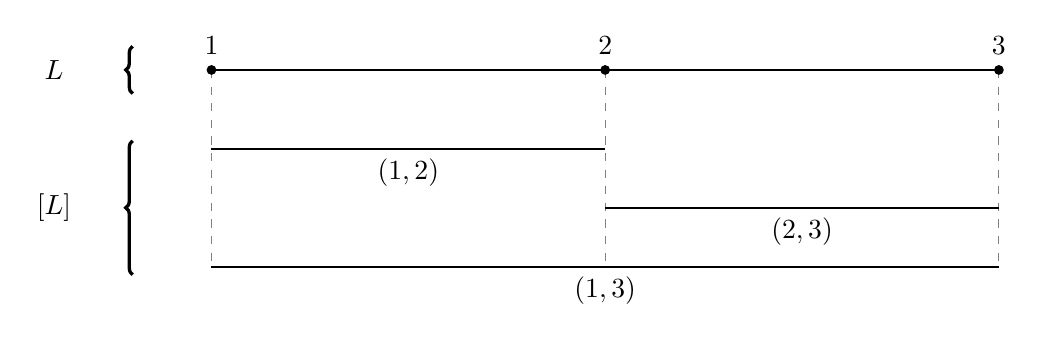
\begin{tikzpicture}
    \draw[dashed, color=gray, -] (0,0)     -- (0, -2.5);
    \draw[dashed, color=gray, -] (5,0)     -- (5, -2.5);
    \draw[dashed, color=gray, -] (10,0) -- (10, -2.5);

    \draw [thin,-] (0,0) -- (10,0);
    \node[circle,fill,inner sep=1.25pt,label=above:$1$] (1) at (0,0)  {};
    \node[circle,fill,inner sep=1.25pt,label=above:$2$] (2) at (5,0)  {};
    \node[circle,fill,inner sep=1.25pt,label=above:$3$] (3) at (10,0) {};

    \draw[thick, -] (0,-1)    -- (5,-1)     node[below, midway] {$(1,2)$};
    \draw[thick, -] (5,-1.75) -- (10,-1.75) node[below, midway] {$(2,3)$};
    \draw[thick, -] (0,-2.5)  -- (10,-2.5)  node[below, midway] {$(1,3)$};

    \node (L)      at (-2, 0)     {$L$};
    \node (interL) at (-2, -1.75) {$\inter[L]$};
    \draw [very thick,decorate,decoration = {brace}] (-1,-0.3) -- (-1,0.3);
    \draw [very thick,decorate,decoration = {brace}] (-1,-2.6) -- (-1,-0.9);
  \end{tikzpicture}
  \caption{An example of the $\inter$ construction}
  \label{fig:inter_example}
\end{figure}

Given an adjunction, it is always helpful to compute the associated unit and counit natural
transformations. In our case, the unit is a natural transformation
$\unit{} : \id{\aias} \to \inter[\points]$
whose component at an interval algebra $A$ is given by
$\unit{A} = \phi_{A,\points[A]}(\id{\points[A]})$. Computing this, we get the map
\begin{equation*}
  \unit{A} : A \to \inter[\points[A]] \text{ sending } I \mapsto (\istart{I}, \iend{I})
\end{equation*}
Dually, the counit here is a natural transformation $\counit{} : \points[\inter] \to \id{\slos}$
where each of its components is given by $\counit{L} = \psi_{\inter[L],L}(\id{\inter[L]})$.
Fixing some $L$ and working through this construction, we get
\begin{equation*}
  \counit{L} : \points[\inter[L]] \to L \text{ sending }
    \istart{(a,b)} \mapsto a \text{ and } \iend{(a,b)} \mapsto b
\end{equation*}

\begin{prop}
The counit component at a strict linear order $L$, $\counit{L}$, is an isomorphism if and only if
$|L| \neq 1$.
\end{prop}
\begin{proof}
  First, suppose that $|L|=1$, so $L = \{a\}$. Then $\inter[L] = \emptyset$ as we do not allow empty
  intervals and so $\points[\inter[L]] = \emptyset$ too. As such, $\counit{L}$ cannot be an
  isomorphism.

  For the converse, first notice that $\counit{L}$ is a map in $\slos$, hence it must be injective.
  Provided that $|L| \neq 1$ then it also turns out to be surjective: fix some
  $a \in L$, there must be at least one distinct $b \in L$. Now either $a < b$, so $(a,b)$ is a
  valid interval over $L$ and then $\counit{L}(\istart{(a,b)}) = a$. Alternatively, $b < a$, so
  $(b, a)$ is an interval in $\inter[L]$ and $\counit{L}(\iend{(b,a)}) = a$
\end{proof}

As for the unit, it will give us an isomorphism when our interval algebra already has all possible
intervals. More precisely, the unit is an isomorphism when it is of the form $\inter[L]$ for some
linear order $L$.

\begin{prop}
  The unit component at an interval algebra $A$, $\unit{A}$, is an isomorphism if and only if
  $A$ is isomorphic to $\inter[L]$ for some $L$.
\end{prop}
\begin{proof}
  First, if $\unit{A}$ is an isomorphism, then we can set $L = \points[A]$ and $A \cong \inter[L]$.

  For the converse, fix some isomorphism $f : A \to \inter[L]$ for some linear order $L$. If $L$ has
  a single element, then $\inter[L] = \emptyset = \inter[\emptyset]$, so we can always assume that
  $|L| \neq 1$ and that $\counit{L}$ is an isomorphism. Consider the composite
  \begin{equation*}
    \inter[\counit{L} \circ \points[f]] \circ \unit{A} \circ f^{-1} : \inter[L] \to \inter[L]
  \end{equation*}
  This will send an element $(a,b) \in \inter[L]$ to
  \begin{align*}
    \inter[\counit{L} \circ \points[f]] \circ \unit{A} \circ f^{-1}(a,b)
      & = \inter[\counit{L} \circ \points[f]]\left( \istart{f^{-1}(a,b)}
                                                  , \iend{f^{-1}(a,b)}
                                             \right) \\
      & = \left( \counit{L} \circ \points[f] (\istart{f^{-1}(a,b)})
               , \counit{L} \circ \points[f] (\iend{f^{-1}(a,b)})
          \right) \\
      & = \left( \counit{L}(\istart{(a,b)})
               , \counit{L}(\iend{(a,b)})
          \right) \\
      & = (a,b)
  \end{align*}
  That is, the above composite is the identity map on $\inter[L]$. Since $f$ and $\counit{L}$ are
  isomorphisms, then $\inter[\counit{L} \circ \points[f]]$ is also an isomorphism. As a result,
  $\unit[A]$ must also be an isomorphism as desired.
\end{proof}

The condition for the unit to be an isomorphism may not be as explicit as for the counit, but it
can still be useful. In the finite case we have
$|\inter[L]| = \binom{|L|}{2} = \frac{|L|(|L|-1)}{2}$, which is an increasing function in $|L|$.
Going over the first few values we then see that $|\inter[L]|$ cannot be 2,4 or 5, which means that
any interval algebra $A$ with 2,4 or 5 elements must be missing intervals, and as such $\unit{A}$
will be only injective, but not surjective.

\begin{cor}
  There exists an equivalence of categories between the full subcategory of strict linear orders $L$
  with $|L| \neq 1$ and the full subcategory of interval algebras of the form $\inter[L]$.
\end{cor}
\begin{proof}
  An adjunction can always be restricted to an equivalence of categories by considering the full
  subcategories where the unit and counit are isomorphisms.
\end{proof}

% {\color{blue} TODO: consider what our functors do to elementary embeddings?}

\newpage
\section{The Model Theory of Interval Algebras}
\label{sec:model_theory}

\subsection{The Fraïssé Limit of the Finite Interval Algebras}

We start by considering the class $\finaia$ of finite interval algebras. From our work in
\cref{ssub:homogeneous_structures_and_fraisse_classes}, we know that $\finaia$ satisfies the HP,
since $\taia$ is universal and relational. $\laia$ is also finite, so $\finaia$ must be EC.

To prove that $\finaia$ has the JEP and AP, notice that $\points$ must send finite interval algebras
to finite strict linear orders. In fact, given an interval algebra $A$, $|\points[A]| \leq 2|A|$
since $\points[A]$ is a quotient of $A + A$. Similarly, $\inter$ must also send finite strict linear
orders to finite interval algebras as given a strict linear order $L$,
$|\inter[L]| = \binom{|L|}{2}$. Using this fact, we will be able to reduce the proof of these
properties to the proof that $\finslo$ satisfies them.

\begin{prop}
  The class $\finaia$ has the joint embedding property.
\end{prop}
\begin{proof}
  Given two finite interval algebras $A$ and $B$, we use the JEP of strict
  linear orders to get the following diagram in $\slos$
  \[\begin{tikzcd}
    {\points[A]} \\
    && \Omega \\
    {\points[B]}
    \arrow["f", from=1-1, to=2-3]
    \arrow["g"', from=3-1, to=2-3]
  \end{tikzcd}\]
  Then, applying $\inter$ and using the adjunction unit $\eta$, we get
  % https://q.uiver.app/?q=WzAsNSxbMiwwLCJcXGludGVyW1xccG9pbnRzW0FdXSJdLFsyLDIsIlxcaW50ZXJbXFxwb2ludHNbQl1dIl0sWzQsMSwiXFxpbnRlcltcXE9tZWdhXSJdLFswLDAsIkEiXSxbMCwyLCJCIl0sWzAsMiwiXFxpbnRlcltmXSIsMCx7ImNvbG91ciI6WzAsNjAsNjBdfSxbMCw2MCw2MCwxXV0sWzEsMiwiXFxpbnRlcltnXSIsMix7ImNvbG91ciI6WzAsNjAsNjBdfSxbMCw2MCw2MCwxXV0sWzQsMSwiXFx1bml0e0J9IiwyXSxbMywwLCJcXHVuaXR7QX0iXV0=
  \[\begin{tikzcd}
    A && {\inter[\points[A]]} \\
    &&&& {\inter[\Omega]} \\
    B && {\inter[\points[B]]}
    \arrow["{\inter[f]}", color={rgb,255:red,214;green,92;blue,92}, from=1-3, to=2-5]
    \arrow["{\inter[g]}"', color={rgb,255:red,214;green,92;blue,92}, from=3-3, to=2-5]
    \arrow["{\unit{B}}"', from=3-1, to=3-3]
    \arrow["{\unit{A}}", from=1-1, to=1-3]
  \end{tikzcd}\]
  And the composites $\inter[f] \circ \unit{A}$ and $\inter[g] \circ \unit{B}$ along with
  the interval algebra $\Omega$ give us the joint embedding of $A$ and $B$.
\end{proof}

\begin{prop}
  The class $\finaia$ has the amalgamation property.
\end{prop}
\begin{proof}
  Suppose we have the following diagram in $\aias$
  % https://q.uiver.app/?q=WzAsNCxbMiwwLCJBIl0sWzIsMiwiQiJdLFswLDEsIkMiXSxbNCwxXSxbMiwwLCJmIl0sWzIsMSwiZyIsMl1d
  \[\begin{tikzcd}
    && A \\
    C &&&& {} \\
    && B
    \arrow["f", from=2-1, to=1-3]
    \arrow["g"', from=2-1, to=3-3]
  \end{tikzcd}\]
  Applying $\points$ takes us to $\slos$, at which point we can use the AP of strict linear
  orders to get the commuting square
  % https://q.uiver.app/?q=WzAsNCxbMiwwLCJcXHBvaW50c1tBXSJdLFsyLDIsIlxccG9pbnRzW0JdIl0sWzAsMSwiXFxwb2ludHNbQ10iXSxbNCwxLCJcXE9tZWdhIl0sWzIsMCwiXFxwb2ludHNbZl0iLDAseyJjb2xvdXIiOlswLDYwLDYwXX0sWzAsNjAsNjAsMV1dLFsyLDEsIlxccG9pbnRzW2ddIiwyLHsiY29sb3VyIjpbMCw2MCw2MF19LFswLDYwLDYwLDFdXSxbMCwzLCJmJyJdLFsxLDMsImcnIiwyXV0=
  \[\begin{tikzcd}
    && {\points[A]} \\
    {\points[C]} &&&& \Omega \\
    && {\points[B]}
    \arrow["{\points[f]}", color={rgb,255:red,214;green,92;blue,92}, from=2-1, to=1-3]
    \arrow["{\points[g]}"', color={rgb,255:red,214;green,92;blue,92}, from=2-1, to=3-3]
    \arrow["{f'}", from=1-3, to=2-5]
    \arrow["{g'}"', from=3-3, to=2-5]
  \end{tikzcd}\]
  Now going back to $\aias$ gives the commuting diagram
  % https://q.uiver.app/?q=WzAsOSxbNCwwLCJcXGludGVyW1xccG9pbnRzW0FdXSJdLFs0LDIsIlxcaW50ZXJbXFxwb2ludHNbQl1dIl0sWzIsMSwiXFxpbnRlcltcXHBvaW50c1tDXV0iXSxbNiwxLCJcXGludGVyW1xcT21lZ2FdIl0sWzAsMSwiQyJdLFswLDBdLFsxLDBdLFsyLDAsIkEiXSxbMiwyLCJCIl0sWzIsMCwiXFxpbnRlcltcXHBvaW50c1tmXV0iLDEseyJjb2xvdXIiOlswLDYwLDYwXX0sWzAsNjAsNjAsMV1dLFsyLDEsIlxcaW50ZXJbXFxwb2ludHNbZ11dIiwxLHsiY29sb3VyIjpbMCw2MCw2MF19LFswLDYwLDYwLDFdXSxbMCwzLCJcXGludGVyW2YnXSIsMCx7ImNvbG91ciI6WzAsNjAsNjBdfSxbMCw2MCw2MCwxXV0sWzEsMywiXFxpbnRlcltnJ10iLDIseyJjb2xvdXIiOlswLDYwLDYwXX0sWzAsNjAsNjAsMV1dLFs4LDEsIlxcdW5pdHtCfSIsMl0sWzcsMCwiXFx1bml0e0F9Il0sWzQsMiwiXFx1bml0e0N9IiwxXSxbNCw3LCJmIl0sWzQsOCwiZyIsMl1d
  \[\begin{tikzcd}
    {} & {} & A && {\inter[\points[A]]} \\
    C && {\inter[\points[C]]} &&&& {\inter[\Omega]} \\
    && B && {\inter[\points[B]]}
    \arrow["{\inter[\points[f]]}"{description}, color={rgb,255:red,214;green,92;blue,92}, from=2-3, to=1-5]
    \arrow["{\inter[\points[g]]}"{description}, color={rgb,255:red,214;green,92;blue,92}, from=2-3, to=3-5]
    \arrow["{\inter[f']}", color={rgb,255:red,214;green,92;blue,92}, from=1-5, to=2-7]
    \arrow["{\inter[g']}"', color={rgb,255:red,214;green,92;blue,92}, from=3-5, to=2-7]
    \arrow["{\unit{B}}"', from=3-3, to=3-5]
    \arrow["{\unit{A}}", from=1-3, to=1-5]
    \arrow["{\unit{C}}"{description}, from=2-1, to=2-3]
    \arrow["f", from=2-1, to=1-3]
    \arrow["g"', from=2-1, to=3-3]
  \end{tikzcd}\]
  For the AP of the finite interval algebras, we are only interested in the outer square. The
  necessary maps are then $\inter[f'] \circ \unit{A}$ and $\inter[g'] \circ \unit{B}$, both
  mapping into $\inter[\Omega]$.
\end{proof}

\begin{thm}
  The Fraïssé limit of $\finaia$ is $\inter[\Q]$
\end{thm}
\begin{proof}
  To show that the Fraïssé limit of the finite interval algebras is $\inter[\Q]$, it suffices to
  show that $\age(\inter[\Q]) = \finaia$ and that $\inter[\Q]$ is homogeneous.

  To see that $\age(\inter[\Q]) = \finaia$, prove that both sides include into the other.
  Suppose we have some finitely generated $\laia$-substructure $A \subset \inter[\Q]$. Since
  $\taia$ is universal, $A$ must also be an interval algebra. Furthermore, since $\laia$ is
  relational, $A$ must also be finite, so $A \in \finaia$. For the converse inclusion, consider
  some finite interval algebra $A$, it must embed into $\inter[\points[A]]$, which in turn
  embeds into $\inter[\Q]$ (since $\points[A]$ is finite, hence embeddable into $\Q$).
  Restricting these composition of these embeddings onto their image in $\inter[\Q]$ then gives
  the needed isomorphism.

  As for why $\inter[\Q]$ is homogeneous, fix two $\laia$-substructures $A,B \subseteq \inter[\Q]$,
  along with some $\laia$-isomorphism $f : A \to B$. In essence we have the following
  diagram of interval algebras, where $i$ and $j$ are the inclusions into $\inter[\Q]$:
  % https://q.uiver.app/?q=WzAsNCxbMCwyLCJBIl0sWzIsMiwiQiJdLFswLDAsIlxcaW50ZXJbXFxRXSJdLFsyLDAsIlxcaW50ZXJbXFxRXSJdLFswLDEsImYiXSxbMCwyLCJpIl0sWzEsMywiaiIsMl1d
  \[\begin{tikzcd}
    {\inter[\Q]} && {\inter[\Q]} \\
    \\
    A && B
    \arrow["f", from=3-1, to=3-3]
    \arrow["i", from=3-1, to=1-1]
    \arrow["j"', from=3-3, to=1-3]
  \end{tikzcd}\]
  Applying $\inter$ to move to linear orders, we can postcompose $\points[i]$ and $\points[j]$ with
  the counit at $\Q$ to realise $\points[A]$ and $\points[B]$ as $\lslo$-substructures of $\Q$.
  Now, $\points[f]$ is still an isomorphism as these are preserved by functors, and using the
  fact that $\Q$ is homogeneous, we can extend $\points[f]$ to an isomorphism $g$, giving the
  commuting diagram
  % https://q.uiver.app/?q=WzAsNyxbMCw0LCJcXHBvaW50c1tBXSJdLFsyLDQsIlxccG9pbnRzW0JdIl0sWzAsMiwiXFxwb2ludHNbXFxpbnRlcltcXFFdXSJdLFsyLDIsIlxccG9pbnRzW1xcaW50ZXJbXFxRXV0iXSxbMCwwLCJcXFEiXSxbMiwwLCJcXFEiXSxbMCwxXSxbMCwxLCJcXHBvaW50c1tmXSIsMCx7ImNvbG91ciI6WzAsNjAsNjBdfSxbMCw2MCw2MCwxXV0sWzAsMiwiXFxwb2ludHNbaV0iLDAseyJjb2xvdXIiOlswLDYwLDYwXX0sWzAsNjAsNjAsMV1dLFsyLDQsIlxcY291bml0e1xcUX0iXSxbMyw1LCJcXGNvdW5pdHtcXFF9IiwyXSxbMSwzLCJcXHBvaW50c1tqXSIsMix7ImNvbG91ciI6WzAsNjAsNjBdfSxbMCw2MCw2MCwxXV0sWzQsNSwiZyJdXQ==
  \[\begin{tikzcd}
    \Q && \Q \\
    {} \\
    {\points[\inter[\Q]]} && {\points[\inter[\Q]]} \\
    \\
    {\points[A]} && {\points[B]}
    \arrow["{\points[f]}", color={rgb,255:red,214;green,92;blue,92}, from=5-1, to=5-3]
    \arrow["{\points[i]}", color={rgb,255:red,214;green,92;blue,92}, from=5-1, to=3-1]
    \arrow["{\counit{\Q}}", from=3-1, to=1-1]
    \arrow["{\counit{\Q}}"', from=3-3, to=1-3]
    \arrow["{\points[j]}"', color={rgb,255:red,214;green,92;blue,92}, from=5-3, to=3-3]
    \arrow["g", from=1-1, to=1-3]
  \end{tikzcd}\]
  Finally, we apply $\inter$ to bring us back to interval algebras, where we have the following
  diagram:
  % If modifying diagram, don't forget to add [scale cd=0.91]
  % https://q.uiver.app/?q=WzAsMTIsWzIsNCwiXFxpbnRlcltcXHBvaW50c1tBXV0iXSxbNCw0LCJcXGludGVyW1xccG9pbnRzW0JdXSJdLFsyLDIsIlxcaW50ZXJbXFxwb2ludHNbXFxpbnRlcltcXFFdXV0iXSxbNCwyLCJcXGludGVyW1xccG9pbnRzW1xcaW50ZXJbXFxRXV1dIl0sWzIsMCwiXFxpbnRlcltcXFFdIl0sWzQsMCwiXFxpbnRlcltcXFFdIl0sWzQsNiwiQiJdLFsyLDYsIkEiXSxbNiwyLCJcXGludGVyW1xcUV0iXSxbMCwyLCJcXGludGVyW1xcUV0iXSxbMCw0LCJBIl0sWzYsNCwiQiJdLFswLDEsIlxcaW50ZXJbXFxwb2ludHNbZl1dIiwwLHsiY29sb3VyIjpbMCw2MCw2MF19LFswLDYwLDYwLDFdXSxbMSwzLCJcXGludGVyW1xccG9pbnRzW2ldXSIsMCx7ImNvbG91ciI6WzAsNjAsNjBdfSxbMCw2MCw2MCwxXV0sWzAsMiwiXFxpbnRlcltcXHBvaW50c1tpXV0iLDIseyJjb2xvdXIiOlswLDYwLDYwXX0sWzAsNjAsNjAsMV1dLFsyLDQsIlxcaW50ZXJbXFxjb3VuaXR7XFxRfV0iLDIseyJjb2xvdXIiOlswLDYwLDYwXX0sWzAsNjAsNjAsMV1dLFszLDUsIlxcaW50ZXJbXFxjb3VuaXR7XFxRfV0iLDAseyJjb2xvdXIiOlswLDYwLDYwXX0sWzAsNjAsNjAsMV1dLFs0LDUsIlxcaW50ZXJbZ10iLDAseyJjb2xvdXIiOlswLDYwLDYwXX0sWzAsNjAsNjAsMV1dLFs3LDAsIlxcdW5pdHtBfSIsMl0sWzYsMSwiXFx1bml0e0J9Il0sWzgsMywiXFx1bml0e1xcaW50ZXJbXFxRXX0iXSxbOSwyLCJcXHVuaXR7XFxpbnRlcltcXFFdfSIsMl0sWzgsNSwiXFxpZHtcXGludGVyW1xcUV19IiwyLHsiY3VydmUiOjN9XSxbOSw0LCJcXGlke1xcaW50ZXJbXFxRXX0iLDAseyJjdXJ2ZSI6LTN9XSxbNyw2LCJmIiwyXSxbMTAsOSwiaSJdLFsxMCwwLCJcXHVuaXR7QX0iLDJdLFs3LDEwLCJcXGlke0F9IiwwLHsiY3VydmUiOi0zfV0sWzExLDgsImoiLDJdLFsxMSwxLCJcXHVuaXR7Qn0iXSxbNiwxMSwiXFxpZHtCfSIsMix7ImN1cnZlIjozfV1d
  \[\begin{tikzcd}[scale cd=0.91]
    && {\inter[\Q]} && {\inter[\Q]} \\
    \\
    {\inter[\Q]} && {\inter[\points[\inter[\Q]]]} && {\inter[\points[\inter[\Q]]]} && {\inter[\Q]} \\
    \\
    A && {\inter[\points[A]]} && {\inter[\points[B]]} && B \\
    \\
    && A && B
    \arrow["{\inter[\points[f]]}", color={rgb,255:red,214;green,92;blue,92}, from=5-3, to=5-5]
    \arrow["{\inter[\points[i]]}", color={rgb,255:red,214;green,92;blue,92}, from=5-5, to=3-5]
    \arrow["{\inter[\points[i]]}"', color={rgb,255:red,214;green,92;blue,92}, from=5-3, to=3-3]
    \arrow["{\inter[\counit{\Q}]}"', color={rgb,255:red,214;green,92;blue,92}, from=3-3, to=1-3]
    \arrow["{\inter[\counit{\Q}]}", color={rgb,255:red,214;green,92;blue,92}, from=3-5, to=1-5]
    \arrow["{\inter[g]}", color={rgb,255:red,214;green,92;blue,92}, from=1-3, to=1-5]
    \arrow["{\unit{A}}"', from=7-3, to=5-3]
    \arrow["{\unit{B}}", from=7-5, to=5-5]
    \arrow["{\unit{\inter[\Q]}}", from=3-7, to=3-5]
    \arrow["{\unit{\inter[\Q]}}"', from=3-1, to=3-3]
    \arrow["{\id{\inter[\Q]}}"', curve={height=18pt}, from=3-7, to=1-5]
    \arrow["{\id{\inter[\Q]}}", curve={height=-18pt}, from=3-1, to=1-3]
    \arrow["f"', from=7-3, to=7-5]
    \arrow["i", from=5-1, to=3-1]
    \arrow["{\unit{A}}"', from=5-1, to=5-3]
    \arrow["{\id{A}}", curve={height=-18pt}, from=7-3, to=5-1]
    \arrow["j"', from=5-7, to=3-7]
    \arrow["{\unit{B}}", from=5-7, to=5-5]
    \arrow["{\id{B}}"', curve={height=18pt}, from=7-5, to=5-7]
  \end{tikzcd}\]
  Although not obvious at first, the above diagram commutes, to check this we look at all the
  "irreducible components" individually:
  \begin{itemize}
    \item The middle rectangle in red commutes since it already commuted for linear orders.
    \item The top triangles commute by triangle identities of our adjunction.
    \item The squares to the left, right and bottom of the red rectangle commute by naturality
      of the unit.
    \item The bottom triangles commute due to the use of the identity.
  \end{itemize}
  Chasing around the outside of the diagram, we see that
  \begin{equation*}
    \inter[g] \circ \id{\inter[\Q]} \circ i \circ \id{A} =
      \id{\inter[\Q]} \circ j \circ \id{B} \circ f
  \end{equation*}
  Simplifying by removing identities shows that $\inter[g] \circ i = j \circ f$. Now, since $g$
  was an isomorphism, so is $\inter[g]$, so we have successfully extended $f$ to an
  automorphism of $\inter[\Q]$.
\end{proof}

% {\color{blue} TODO Fraisse Limits can be seen as a type of colimit, check if there is anything
% interesting/noteworthy to say here -- left adjoints only preserve limits generally, but here we
% have a colimit being preserved by a left adjoint (Int(-))}
% Fraisse Limits can be seen as a type of colimit, look into this?
% It's interesting that this colimit is preserved by a right adjoint, namely Int(-)
% WARNING: Not sure if the following makes any sense, I am quite tired -- I suspect my reasoning is
% somewhat flawed though?
% I guess it happens since Pts(Int(-)) is naturally isomorphic to Id(-),
% So suppose the colimit of some diagram D(-) exists for linear orders,
% then if the colimit of Pts(D(-)) exists, it must be isomorphic to the Pts(colimit of D(-))
% This is because left adjoints preserve colimits, so Int(colimit of Pts(D(-))) is the colimit of
% Int(Pts(D(-))), and since Ints(Pts(D(-))) is naturally isomorphic to D(-), the colimit of
% Int(Pts(D(-))) must also be isomorphic to the colimit of D(-)

\subsection*{The Classification theory of Interval Agebras}

\begin{thm}
  An interval algebra $A$ is stable if and only if it is finite.
\end{thm}
\begin{proof}
  % TODO look at exercise 5.5.6 of marker for the order property.
  Suppose that $A$ is an interval algebra and consider the formula
  \begin{equation*}
    \lexord(I, J) = (I \before J) \lor (I \meets J) \lor (I \overlaps J) \lor (I \starts J)
                                  \lor (I \finishedby J) \lor (I \contains J)
  \end{equation*}
  The above formula takes the elements of $A$ and lexicographically orders them, by first comparing
  the start times of each interval, followed by the end times in case the start times align. As a
  result, the formula $\lexord$ induces the structure of a strict linear order on the elements
  of $A$:
  \begin{itemize}
    \item \textbf{irreflexivity}: Fix some interval $I \in A$, then $I = I$. Since the relational
      symbols of interval algebras along with equality are all mutually exclusive,
      neither $I \aiaarrow{i} I$ nor $I \raiaarrow{i} I$ can hold for any $i \in \aiaindex$. This
      means $A \models \lnot \lexord(I, I)$ so $\lexord$ is irreflexive.
    \item \textbf{transitivity}: Fix three intervals $I,J,K \in A$ and suppose that
      $A \models \lexord(I,J)$ and $A \models \lexord(J,K)$. Since $\lexord$ consists of the disjunction of 6
      relational symbols, there are 36 cases which would lead to this situation. Considering each of
      these cases individually and looking up our transitivity axioms for interval algebras, we can
      find all possible relations between $I$ and $K$, which is detailed in \cref{tab:lexord_trans}.
      In all of these cases, we must still have $A \models \lexord(I,K)$, so
      $\lexord$ is transitive.
    \item \textbf{trichotomy}: Fix two intervals $I, J \in A$. First notice that
      \begin{equation*}
        A \models \lexord(J,I) \iff
        (I \after J) \lor (I \metby J) \lor (I \overlappedby J) \lor (I \startedby J)
                      \lor (I \finishes J) \lor (I \contained J)
      \end{equation*}
      Hence $A \models \lexord(I,J) \lor (I = J) \lor \lexord(J,I)$ is equivalent to saying that
      the interval algebra relations are exhaustive, which is one of our axioms. Hence the strict
      ordering given by $\lexord$ is linear.
  \end{itemize}

  \transreltable{lexord_trans}{Cases for transitivy of $\lexord$.}{
    \llrow & \slrow \\
    \lmrow & \smrow \\
    \lorow & \sorow \\
    \lsrow & \ssrow \\
    \lFrow & \sFrow \\
    \lDrow & \sDrow \\
    \hline
    \mlrow & \Flrow \\
    \mmrow & \Fmrow \\
    \morow & \Forow \\
    \msrow & \Fsrow \\
    \mFrow & \FFrow \\
    \mDrow & \FDrow \\
    \hline
    \olrow & \Dlrow \\
    \omrow & \Dmrow \\
    \oorow & \Dorow \\
    \osrow & \Dsrow \\
    \oFrow & \DFrow \\
    \oDrow & \DDrow \\
  }

  Now for any finite interval algebra $A$, all strict linear orders interpretable in $A$ will be
  bounded in size by $|A^k|$ for some $k \in \N$. In particular, all such linear orders must be
  finite, so $A$ is stable.

  For the converse, suppose $A$ is stable. Using $\lexord$ we can linearly order all the elements
  of $A$, but as $A$ is stable this linear order must be finite, hence $A$ must be finite.
\end{proof}

\begin{thm}
  For any linear order $L$, the interval algebra $\inter[L]$ is NIP.
\end{thm}
\begin{proof}
\end{proof}

\begin{exmp}
  Construct an interval algebra with the IP.
\end{exmp}